\documentclass{article}


\usepackage[final]{neurips}
\usepackage[utf8]{inputenc} % allow utf-8 input
\usepackage[T1]{fontenc}    % use 8-bit T1 fonts
\usepackage{hyperref}       % hyperlinks
\usepackage{url}            % simple URL typesetting
\usepackage{booktabs}       % professional-quality tables
\usepackage{amsfonts}       % blackboard math symbols
\usepackage{nicefrac}       % compact symbols for 1/2, etc.
\usepackage{microtype}      % microtypography
\usepackage{graphicx}
\usepackage{subcaption}
\usepackage{wrapfig}
\usepackage{float}
\usepackage{ragged2e}
\usepackage{amsmath}
\usepackage{mathtools}
\usepackage{booktabs}
\usepackage{caption}
\usepackage{float}
\usepackage{titlesec}
\usepackage{capt-of}
\usepackage{array}
\usepackage{arydshln}
\usepackage{xepersian}
\settextfont{XB Yas.ttf}
\setlength\dashlinedash{0.2pt}
\setlength\dashlinegap{1.5pt}
\setlength\arrayrulewidth{0.3pt}

%Widows & Orphans & Penalties

\widowpenalty500
\clubpenalty500
\clubpenalty=9996
\exhyphenpenalty=50 %for line-breaking at an explicit hyphen
\brokenpenalty=4991
\predisplaypenalty=10000
\postdisplaypenalty=1549
\displaywidowpenalty=1602
\floatingpenalty = 20000
\renewcommand{\bibsection}{}

\title{پرسش و پاسخ تصویری در فارسی}

\author{%
  مریم سادات هاشمی \\
  دانشکده مهندسی کامپیوتر\\
  دانشگاه علم و صنعت ایران\\
  \texttt{m\_hashemi94@cs.iust.ac.ir} \\
   \And
    علیرضا اصغری \\
   دانشکده مهندسی کامپیوتر\\
   دانشگاه علم و صنعت ایران\\
    \texttt{a\_asghari@comp.iust.ac.ir}
}


\begin{document}


\begin{minipage}{0.1\textwidth}% adapt widths of minipages to your needs
\includegraphics[width=1.1cm]{iust_logo.png}
\end{minipage}%
\hfill%
\begin{minipage}{0.9\textwidth}\raggedleft
دانشگاه علم و صنعت ایران\\
یادگیری عمیق (بهار ۱۳۹۹)\\
\end{minipage}


\makepertitle

\input{abstract}
\input{intro}
\input{background}
\section{مدل پیشنهاد شده}
{
	در این بخش ابتدا نحوه‌ی آماده‌سازی مجموعه‌داده را توضیح می‌دهیم و سپس به شرح روش‌های پیاده‌سازی شده در این پروژه می‌پردازیم.
	
	\subsection{تهیه‌ی مجموعه‌داده}
	{
		مجموعه‌داده‌ای که برای حل این مسئله انتخاب کردیم؛ مجموعه داده
		 \href{https://visualqa.org/vqa_v1_download.html}{\lr{VQA v1}} 
		 است. مشخصات کامل مجموعه داده را می‌توانید در جدول 1 مشاهده کنید.
		 \begin{table}
			 \begin{center}
			 	\begin{tabular}{ c c c c } 
			 		\hline
			 		& \textbf{تعداد تصاویر} & \textbf{تعدادسوالات} & \textbf{تعداد پاسخ‌ها} \\
			 		\hline \hline
			 		\textbf{داده‌های آموزشی} & 82,783 & 248,349 &  2,483,490 \\
					
					\textbf{داده‌های ارزیابی} & 40,504 & 121,512 & 1,215,120 \\
					
					\textbf{داده‌های تست} & 81,434 & 244,302 & \\
					\hline
			 	\end{tabular}
			 \end{center}
		 \caption{مشخصات مجموعه‌داده VQA}
	 	\end{table}
		برای ترجمه مجموعه‌داده از دو ابزار Google‌ و ترگمان استفاده کردیم. در این مجموعه‌داده برای هر تصویر سه سوال وچود دارد و برای هر سوال 10 پاسخ موجود می‌باشد. در این مجموعه‌داده سه نوع سوال وجود دارد. نوع اول بله و خیر است. نوع دوم تعداد یک شی در تصویر است و نوع سوم مربوط به سوالات دیگر است. توزیع طول سوالات و پاسخ‌ها و 30 پاسخ پرتکرار در این مجموعه‌داده را برای دو حالت ترجمه Google‌‌ و ترگمان را در شکل های 
		\ref{fig:9}
		،
		\ref{fig:10}
		و 
		\ref{fig:11}
		می‌توانید مشاهده کنید. 
	}
	\subsection{\lr{LSTM Q + norm I} \cite{antol2015vqa}}
	{
		\begin{figure}[h]
			\centering
			\includegraphics[scale=0.4]{images/Vanilla_Network.jpg}
			\caption{ساختار کلی روش \lr{LSTM Q + norm I}  .}
			\label{fig:3}
		\end{figure}
		این روش ساده‌ترین روش یادگیری عمیق برای حل مسئله پرسش و پاسخ تصویری است. در اینجا مسئله VQA به عنوان یک مسئله طبقه‌بندی در نظر گرفته می‌شود که در آن 1000 پاسخ پرتکرار به عنوان کلاس‌ها انتخاب می‌شوند.  ساختار کلی این شبکه در شکل 
		\ref{fig:3}
		نشان داده شده است. ابتدا با عبور دادن تصاویر از شبکه 
		\lr{VGG19}
		 برای هر تصویر یک بردار ویژگی 4096تایی در لایه‌ی ماقبل آخر در شبکه‌ی
		  \lr{VGG19}
		   تولید می‌شود. از طرفی دیگر با عبور سوال‌ها از لایه‌یEembedding برای هر کلمه موجود در سوال یک بردار 300تایی تولید می‌شود. سپس از طریق 2 لایه LSTM بردار ویژگی معنایی سوال استخراج  می‌شود. هر یک از بردارهای ویژگی تصویر و سوال را به یک لایه‌ی Dense  1024 واحدی می‌دهیم تا ابعاد بردار‌ها مشابه هم شوند. برای ترکیب بردار ویژگی سوال و تصویر از ضرب نقطه‌ای استفاده می‌کنیم. از این بردار ترکیب شده به عنوان ورودی برای لایه‌ی کاملا متصل استفاده می‌کنیم و در نهایت با عبور از یک لایه softmax کلاس(پاسخ) پیش‌بینی شده بدست می‌آید.
	}

	\subsection{\lr{Stacked Attention Network} \cite{yang2016stacked} }
	{
		ایده‌ی اصلی روش SAN‌ این است که ابتدا از سوال، یک  بازنمایی معنایی و مفهومی استخراج می‌کند. سپس از آن به عنوان یک کوئری برای پیدا کردن مناطقی از تصویر که مرتبط با سوال است؛ استفاده می‌کند. غالباً در مسئله VQA نیاز است تا چندین مرحله استدلال صورت بگیرد. بنابراین در این شبکه از چندین لایه برای جستجو در تصویر استفاده می‌کنیم تا به تدریج به جواب مورد نظر برسیم. ساختار کلی شبکه SAN را در شکل 
		\ref{fig:1}
		می‌توانید مشاهده کنید. شبکه SAN از سه جز اصلی تشکیل شده است: 1) مدل تصویر که با استفاده از CNN ویژگی‌های سطح بالایی را از تصویر استخراج می‌کند. 2) مدل سوال که با استفاده از CNN یا LSTM ویژگی‌های معنایی سوال را استخراج می‌کند. 3) مدل
		 \lr{stacked attention}
		 ‌ که از طریق استدلال چند مرحله‌ای مناطقی از تصویر که مرتبط به سوال است را پیدا می‌کند تا پاسخ را پیش‌بینی کند.
		\begin{figure}[H]
			\centering
			\includegraphics[scale=0.5]{images/san.jpg}
			\caption{ساختار کلی روش SAN .}
			\label{fig:1}
		\end{figure}
	
		\subsubsection{مدل تصویر}
		{
			در این بخش برای استخراج ویژگی از شبکه‌ی
			 \lr{VGG16}
			 ‌ استفاده می‌کنیم و ویژگی‌ها را از آخرین لایه‌ی
			 \lr{pooling}
			  ‌شبکه بدست می‌آوریم. ابتدا تمام تصاویر را به
			 \lr{448×448}
			  تغییر سایز می‌دهیم و بعد از این که تابع پیش‌پردازش موجود برای شبکه‌ی 
			 \lr{VGG16}
			   را بر روی تصاویر اعمال کردیم، تصاویر را برای استخراج ویژگی به شبکه می‌دهیم. بنابراین برای هر تصویر یک ویژگی با ابعاد
			 \lr{512×14×14}
			 حاصل می‌شود. در حقیقت، برای هر تصویر به تعداد
			 \lr{14×14}
			 منطقه استخراج می‌شود که هر منطقه به وسیله‌ی یک بردار ویژگی 512تایی بازنمایی می‌شود. برای راحتی، از یک لایه‌ی
			 \lr{Dense}
			 بعد از شبکه‌ی 
			 \lr{VGG16}
			استفاده می‌کنیم تا ابعاد بردار ویژگی مناطق مشابه با ابعاد بردار ویژگی سوال شود.
		}
	
		\subsubsection{مدل سوال}
		{
			\begin{figure}
				\centering
				\includegraphics[scale=0.5]{images/san_cnn.jpg}
				\caption{مدل سوال براساس CNN .}
				\label{fig:2}
			\end{figure}
			برای استخراج ویژگی‌های معنایی از سوال، از هر دو روش  LSTM‌ و CNN یک بعدی استفاده می‌کنیم. در هر دو روش ابتدا سوال را به یک دنباله‌ی عددی تبدیل می‌کنیم و سپس این دنباله‌ها را به یک لایه‌ی Embedding‌ می‌دهیم. در روش
			 LSTM
			خروجی لایه Embedding را به دو لایه‌ی LSTM می‌دهیم و خروجی آخرین لایه‌ی مخفی LSTM را به عنوان بردار ویژگی سوال در نظر می‌گیریم. در روش CNN خروجی Embedding را به سه لایه‌ی کانولوشنی یک بعدی با فیلترهایی با سایز 1، 2، 3 می‌دهیم که به ترتیب ترکیب‌های یک کلمه‌ای ، دو کلمه‌ای و سه کلمه‌ای را برای ما استخراج می‌کند. در نهایت بر روی خروجی هر سه لایه تابع maxpooling  را اعمال می‌کنیم و با قرار دادن این سه خروجی در کنار هم بردار ویژگی سوال بدست می‌آید. شکل 
			\ref{fig:2}
			مدل سوال بر اساس CNN را نشان می‌دهد.
		}
	
		\subsubsection{مدل \lr{stacked attention}}
		{
			در این بخش، مدل
			\lr{stacked attention}
			 با توجه به ماتریس ویژگی تصویر و بردار ویژگی سوال پاسخ را از طریق استدلال چند مرحله‌ای پیش‌بینی می‌کند. در بسیاری  از موارد، یک پاسخ فقط مربوط به یک ناحیه کوچک از تصویر است. بنابراین، استفاده از یک ماتریس ویژگی کلی  برای تصویر می‌تواند به دلیل وجود نویزهای مناطق بی‌ربط  به پاسخ، منجر به نتایج نامطلوبی شود. در عوض، استدلال از طریق چندین لایه توجه، قادر است به تدریج مناطق غیرمرتبط با جواب را فیلتر کند و از ماتریس ویژگی تصویر حذف کند. بدین منظور ماتریس ویژگی تصویر
		 $v_I$
	    و بردار ویژگی سوال
	    $v_Q$
	    ، را به یک لایه Dense می‌دهیم و خروجی این لایه را به یک تابع softmax می‌دهیم تا توزیع توجه را بر روی نواحی تصویر بدست آوریم. بنابراین داریم:
	    \begin{equation}
	    	h_A = tanh (W_{I,A} v_I \oplus (W_{Q,A}v_Q + b_A))
	    \end{equation}
	    \begin{equation}
	    	p_I = softmax(W_Ph_A + b_P)
	    \end{equation}
	    
	    بر اساس توزیع توجه
	     $p_i$
	     ، جمع وزن‌دار بردارهای تصویر را که هر کدام متناظر به یک منطقه هست را محاسبه می‌کنیم. سپس
	     $\tilde{v}_I$
	      را با بردار ویژگی سوال ترکیب می‌کنیم و یک کوئری برای لایه‌ی بعدی توجه ایجاد می‌کنیم.	    
	     \begin{equation}
	      	\tilde{v}_I =\sum_i p_iv_i,
	     \end{equation}
	     \begin{equation}
	        u =\tilde{v}_I + v_Q.
	     \end{equation}
	      این روش را به تعداد k بار تکرار می‌کنیم. در نهایت از u در لایه‌ی k برای پیش‌بینی پاسخ استفاده می‌کنیم:
	     \begin{equation}
	     	p_{ans} =softmax(W_uu^K + b_u)
	     \end{equation}
	     
		}
	}

	\subsection{\lr{HieCoAttention} \cite{lu2016hierarchical}}
	{
		\begin{figure}
			\centering
			\includegraphics[scale=0.6]{images/hiecoattention.JPG}
			\caption{ساختار کلی روش HieCoAttention}
			\label{fig:7}
		\end{figure}
		روش پیشنهاد شده در 
		\cite{lu2016hierarchical}
		دارای دو ویژگی مهم است. ویژگی اول بازنمایی سلسله‌مراتبی سوال و ویژگی دوم مکانیزم coattention می‌باشد. در ادامه این دو خصوصیات را شرح می‌دهیم.
		
		\subsubsection{بازنمایی سلسله‌مراتبی سوال}
		{
			\begin{figure}[h]
				\centering
				\includegraphics[scale=0.5]{images/hierarchical.jpg}
				\caption{بازنمایی سلسله‌مراتبی سوال.}
				\label{fig:4}
			\end{figure}
		
			در این بخش برای هر سوال سه سطح Embedding را محاسبه می‌کنیم. اولین Embedding مربوط به کلمات است که بعد از این‌که سوال را به دنباله‌های عددی تبدیل کردیم؛ با عبور دادن این دنباله‌ها از لایه‌ی Embedding ، بردارهای Embedding‌ کلمات بدست می‌آید. برای محاسبه سطح بعدی Embedding که مربوط به عبارات است از کانولوشن‌های یک بعدی با فیلترهایی با سایز 1، 2 و 3 استفاده می‌کنیم و سپس با اعمال تابع Maxpooling بردار Embedding هر عبارت بوجود می‌آید. در نهایت از Embedding عبارات  برای محاسبه‌ی Embedding  کل سوال استفاده می‌کنیم. این کار توسط یک لایه LSTM انجام می‌شود. بنابراین  برای هر سوال به صورت سلسله‌مراتبی سه سطح Embedding کلمه، عبارت و سوال تولید می‌شود. بازنمایی سلسله‌مراتبی سوال در شکل
			\ref{fig:4}
			 به تصویر کشیده شده است.
		}
		\subsubsection{مکانیزم coattention}
		{
			\begin{figure}
				\centering
				\begin{subfigure}[b]{0.4\textwidth}
					\centering
					\includegraphics[width=0.85\linewidth]{images/parallel.JPG}
					\caption{}
				\end{subfigure}%
				\begin{subfigure}[b]{0.42\textwidth}
					\centering
					\includegraphics[width=0.85\linewidth]{images/alternating.JPG}
					\caption{}
				\end{subfigure}%
				\caption
				{
					(آ) 
					\lr{parallel coattention}
					(ب)
					\lr{alternating coattention}
				}
				\label{fig:5}
			\end{figure}
			در 
			\cite{}
			 دو مکانیزم برای coattention پیشنهاد شده است که از نظر ترتیب تولید 
			\lr{attention map}
			 برای سوال و تصویر با هم تفاوت دارند. اولین مکانیزم که
			\lr{parallel coattention}
			 نامیده می‌شود، باعث تولید attention به طور همزمان برای سوال و تصویر می‌شود. به مکانیزم دوم
			\lr{alternating coattention}
			 می‌گویند که برای تولید attention‌ برای سوال و تصویر به صورت تناوبی عمل می‌کند (شکل 
			\ref{fig:5}
			 ). این مکانیزم coattention در هر سه سطح سلسله‌مراتبی سؤال اجرا می‌شوند.  در این پروژه ما از مکانیزم 
			 \lr{parallel coattention}
			 استفاده می‌کنیم. در این مکانیزم با محاسبه شباهت بین ویژگی‌های تصویر و سوال، تصویر و سؤال را به هم متصل می‌کنیم. اگر بردار ویژگی تصویر را با V و بازنمایی سوال را با Q نشان دهیم؛ ماتریس شباهت C 
			 به صورت زیر محاسبه می‌شود:
			 \begin{equation}
			 	C = tanh(Q^TW_bV)
			 \end{equation}
			 
			 پس از محاسبه ماتریس شباهت، برای محاسبه بردار وزن‌های attention برای تصویر و سوال از روابط زیر استفاده می‌کنیم:
			 \begin{equation}
			 \begin{aligned}
			 	H^v = tanh(W_vV + (W_qQ)C), \ \ \ \ \  H^q = tanh(W_qQ+ (W_vV)CT)\\
			 	a^v = softmax(w^T_{hv}H^v), \ \ \ \ \  a^q = softmax(w^T_{hq}H^q) \ \ \ \ \ \ \ \ \ \ \ \ \ 
			 \end{aligned}
			 \label{eq:1}
			 \end{equation}
			 که در عبارت 
			 \ref{eq:1}
			 $W_v$
			 ، 
			 $W_q$
			 ،
			 $w_{hv}$
			 و
			 $w_{hq}$
			 پارامترهای وزن هستند. 
			 $a_v$
			 و 
			 $a_q$
			 نیز به ترتیب وزن‌های attention برای تصویر و سوال هستند. با توجه به وزن‌های attention ، بردارهای توجه تصویر و سوال به وسیله‌ی جمع وزن‌دار ویژگی‌های تصویر و ویژگی‌های سوال با وزن‌های attention محاسبه می‌شوند:
			 \begin{equation}
			 \hat{v} =\sum_{n+1}^{N} a^v_nv_n,\ \ \ \ \ \hat{q} = \sum_{t=1}^{T}a^q_t q_t
			 \end{equation}
			 
		}
	
		\subsubsection{پیش‌بینی پاسخ}
		{
			\begin{figure}[h]
				\centering
				\includegraphics[scale=0.6]{images/answer.JPG}
				\caption{پیش‌بینی پاسخ}
				\label{fig:6}
			\end{figure}
		
			ما پاسخ را بر اساس coattention تصویر و سوال بدست آمده در هر سه سطح Embedding پیش‌بینی می‌کنیم. از یک پرسپترون چندلایه (MLP) استفاده می‌کنیم تا ویژگی‌های attention را همان طور که در شکل 
		\ref{fig:6}	
			نشان داده شده است؛ ترکیب کنیم.
			\begin{equation}
			\begin{aligned}
			h^w = tanh(W_w(\hat{q}^w + \hat{v}^w))\ \ \ \  \\
			h^p = tanh(W_p[\hat{q}^p + \hat{v}^p), h^w]) \\
			h^s = tanh(W_s[(\hat{q}^s + \hat{v}^s), h^p]) \\
			p = softmax(W_hh^s)  \ \ \ \ \ \ \ \ \ \ \ \ \ 
			\end{aligned}
			\end{equation}
		
			 $W_W$
			 ، 
			 $W_p$
			 ،
			 $W_s$
			  و
			 $W_h$
			  	پارامترهای وزن هستند. p احتمال پاسخ نهایی است.
		}
	}

}


\section{ نتایج و تحلیل}
{  در این بخش ابتدا روش ارزیابی مورد استفاده در این مسئله را بررسی می‌کنیم. سپس به این موضوع می‌پردازیم که مشکل بیش برازش در اینجا چگونه تعریف می‌شود و برای حل آن باید چه کارهایی انجام دهیم. در نهایت نتایج هر کدام از روش‌ها را بررسی خواهیم کرد. دقت شود که در برخی از جدول‌ها از اصلاح hard‌ و soft استفاده شده است. که hard به معنای این است که 
	 \lr{Early stopping}
	  بر اساس خطای داده‌های ارزیابی است و در این حالت مدل حداکثر قدرت خود نخواهد رسید. soft به این معنی است که 
	  \lr{Early stopping}
	  براساس دقت داده‌های ارزیابی است و مدل به حداکثر قدرت خود خواهید رسید. کدهای پروژه را می‌توانید در
	  \href{https://github.com/maryamhashemi/Persian_VQA}{ گیت هاب}
	  مشاهده کنید.
	\subsection{پروتکل ارزیابی}
	{
		در مقاله
		\cite{antol2015vqa}
		، معیار ارزیابی خاصی برای این مساله استفاده شده است. به عبارتی دقت را مانند روش‌های معمول در یادگیری ماشین محاسبه نمی‌کنیم. برای محاسبه دقت ارزیابی پاسخ‌های تولید شده برای سوال (نه انتخاب از بین پاسخ‌های چند گزینه‌ای)   درمجموعه مورد ارزیابی، فرمول زیر را داریم :
		\begin{equation}
		accuracy = min(\frac{\# humans that provided that answer}{3} , 1)
		\label{eq:2}
		\end{equation}
		در مجموعه‌داده اصلی برای داده‌های آموزش و ارزیابی، به ازای هر سوال 10 پاسخ انسانی گردآوری شده است که افراد مختلف به آن سوال با سطوح اطمینان مختلف، پاسخ داده‌اند. حال با توجه به این‌که ما مدل را بر روی مجموعه آموزش، آموزش داده‌ایم و بر روی مجموعه ارزیابی، آن را مورد ارزیابی قرار می‌دهیم، دقت را از این طریق محاسبه می‌کنیم.
		
		طبق این فرمول برای این‌که پاسخ پیش‌بینی شده توسط ماشین به یک سوال کاملا صحیح در نظر گرفته شود، می‌بایست پاسخ ماشین، با پاسخ حداقل 3 عامل انسانی یکسان باشد و در نتیجه امتیاز کامل 1 را از ارزیابی آن سوال دریافت می‌کند. با توجه به فرمول اگر 2 نفر پاسخشان با پاسخ مدل یکی باشد، امتیاز 0.66 و اگر پاسخ مدل تنها با پاسخ یک نفر از آن 10 عامل انسانی یکسان باشد، امتیاز 0.33 دریافت می‌کند.
		
		همانطور که می‌بینیم ارزیابی سهل گیرانه تری نسبت به ارزیابی معمولی یک پاسخ (که وضعیت 0 یا صدی صحت برای آن متصور می‌شود)، معرفی شده‌است.  این روش برای ارزیابی مسئله VQA برای اولین بار در 
		\cite{antol2015vqa}
		معرفی شده است. در حال حاضر که حدود 5 سال از انتشار آن می‌گذرد، قریب به اتفاق مقالات و روش‌های دیگر در این زمینه از این فرمول برای ارزیابی روش یادگیری خود استفاده نموده‌اند و به عنوان فرمولی استاندارد و مناسب به عنوان پروتکل ارزیابی در VQA شناخته شده است.
		
	}

	\subsection{بیش برازش، زمان رخ دادن و حل آن}
	{
		در فاز پیشرفت پروژه، نتایجی که بر روی روش پایه مقاله با داده‌های کم بدست آوردیم؛ نشان از بیش برازش داشت. در این فاز بررسی‌ها و آزمایش‌های متعددی انجام دادیم تا علت مشکل و روش حل آن را بیابیم.
	مقاله
		\cite{ilievski2017simple}
		ریشه این مسئله و رواج داشتن آن به شکل کلی و معمول در VQA را بررسی کرده است.   زمانی که معیار خطا را 
		\lr{cross entropy}
		 در نظر می‌گیریم؛ به صورت سخت‌گیرانه عمل می‌کنیم زیرا اگر پاسخ مدل دقیقا برابر با پاسخ صحیح نباشد، مدل جریمه می‌شود. این در حالی است که عبارت
		\ref{eq:2}
		  از روش سهل گیرانه‌تری استفاده می‌کند. در نتیجه این امر باعث اختلاف بین معیار خطا
		\lr{cross entropy}
		و دقت  مدل می‌شود. در
	    \cite{ilievski2017simple}
		به معرفی معیار خطا
		\lr{soft cross entropy}
		  پرداخته شده است و در محاسبه خطا، تمامی پاسخ‌های انسانی را درنظر می‌گیرد که اختلاف بین رفتار loss و دقت کاهش می‌یابد و همگرایی آموزش مدل نیز بهبود می‌یابد. بنابراین معیار اصلی برای تشخیص بیش برازش، استفاده از عبارت
		  \ref{eq:2}
		 است که به عنوان پروتکل استاندارد ارزیابی در این حوزه شناخته می‌شود. 
		 \begin{figure}[H]
		 	\centering
		 	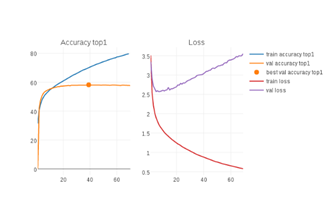
\includegraphics[scale=0.3]{images/i2.jpg}
		 	\caption{}
		 	\label{fig:9}
		 \end{figure}
		 برای مثال در شکل
		  \ref{fig:9}
		  از نظر
		  \lr{cross entropy}
		   بیش برازش داریم اما از نظر پروتکل ارزیابی بیش برازش اتفاق نیفتاده است و بهترین دقت در گام 40 رخ داده است.
		   
		   \begin{figure}[H]
		   	\centering
		   	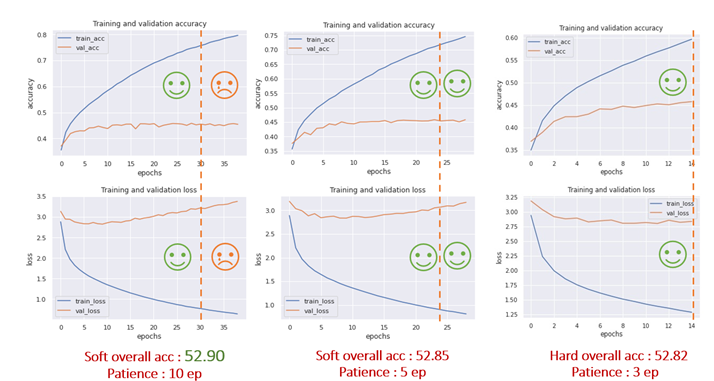
\includegraphics[scale=0.7]{images/i3.png}
		   	\caption{}
		   	\label{fig:10}
		   \end{figure}
	   
		   شکل
		   \ref{fig:10}
		  نتایج سه آزمایشی که با استفاده از 
		  \lr{Early stopping}
		   برمبنای دقت با patience های متفاوت و خطای 
		   \lr{cross entropy}
		   اجرا شده است را نشان می‌دهد. در ستون سمت راست از p برابر با 3 استفاده شده است و یادگیری در گام چهاردهم متوقف شده است. در این آزمایش از نظر خطا، بیش برازشی اتفاق نیفتاده است و به دقت
		   $ 52.82 $
		   رسیده‌ایم. در آزمایش دوم p را بیشتر کرده‌ایم و یادگیری در گام 24 به اتمام می‌رسد.از نظر تابع خطا تا گام 24 هم بیش برازش اتفاق افتاده است. اما دقت بیشتر شده است پس طبق پروتکل بیش برازشی اتفاق نیفتاده است. در ستون سوم با افزایش p یادگیری در گام 30 به پایان می‌رسد و دقت از مرحله قبل  بیشتر شده است. این نشان می‌دهد که در ستون دوم حتی بعد از گام 24 نیز بیش برازش رخ نداده است و تنها جایی که احتمالاً دچار بیش برازش اتفاق افتاده است، از گام 30 به بعد است (چرا که ممکن است اگر p را بیشتر می کردیم سناریوی آزمایش‌های قبل تکرار شود.). در نهایت  بهترین مدل در گام 30 می‌باشد.
		   
 زمانی که مشکل بیش برازش رخ می‌دهد، برای حل آن از نرمالیزه سازی l2 تصاویر، 
  \lr{recurrent dropout}
   و بهینه سازهای متفاوت مثل adam و adadelta  و یا RmsProp‌ با نرخ یادگیری کاهشی استفاده می‌کنیم.
		   
		  
		
	}
	\subsection{\lr{LSTM Q + norm I}}
	{
		آزمایش‌های متعددی برای این روش انجام شده است که جزئیات کامل آن در فایل‌های ضممیه قرار داده شده است. در اینجا به بررسی مهم‌ترین نتایج می‌پردازیم. 
		
		پس از بررسی نتایج آزمایش‌های ضمیمه شده به نتایج زیر دست یافتیم:
		\begin{enumerate}
			\item بهترین بهینه‌ساز adadelta با نرخ یادگیری 1 است که همگرایی مدل را افزایش می‌دهد.
			\item برای پیش پردازش سوال ها از کتابخانه hazm استفاده کرده‌ایم که منجر به افزایش دقت شد و همچنین روش pre در padding عملکرد بهتری از‌ حالت post‌ داشت .
			\item برای embedding سوال‌ها از fasttext‌ استفاده می‌کنیم زیرا عملکرد آن نسبت به Glove بهتر است.
			\item استفاده از \lr{recurrent dropout} به جای dropout معمولی نتایج را بهبود می‌دهد.
			\item استفاده از BatchNormalization‌ دقت‌ مدل را افزایش می‌دهد.
		\end{enumerate}
	
	نتایج این مدل را برای زبان فارسی در جدول 
	\ref{tabel:4}
	می‌توانید مشاهده کنید. در هر دو حالت سخت و نرم دقت برای ترجمه‌های Google بهتر از ترگمان است و همان طور که پیش بینی می‌کردیم دقت مدل‌های نرم بیشتر از مدل‌های سخت است و نشان می‌دهد که مدل از حداکثر ظرفیتش استفاده کرده است.
	
		\begin{table}[H]\centering
			\begin{latin}
				\begin{small}
					\begin{tabular}{ c|| c c c c || c c c c} \toprule
						\multicolumn{1}{c ||}{ }&\multicolumn{4}{c||}{\textbf{Google Translation}} & \multicolumn{4}{c}{\textbf{Targoman Translation}} \\ \midrule
						\textbf{Method} & \textbf{yes/no} & \textbf{Number} & \textbf{Other} & \textbf{All} & \textbf{yes/no} & \textbf{Number} & \textbf{Other} & \textbf{All} \\ \midrule
						\textbf{lstm Q + VGG19(hard)} & 76.14\ & 32.97\ & 35.78\ & 50.53\ & 75.58\ & 32.61\ & 33.53\ & 49.15\ \\
						\textbf{lstm Q + VGG19(soft)} & 76.74\ & 32.5\ & 36.98\ & \textbf{51.3}\ & 76.86\ & 31.85\ & 36.26\ & \textbf{50.91}\ \\
						%\textbf{lstm Q + VGG19} & \ & \ & \ & \ & \ & \ & \ & \ \\
						\bottomrule
					\end{tabular}
				\end{small}
			\end{latin}
			\caption{دقت  روش \lr{baseline} بر روی مجموعه‌داده فارسی تهیه شده.}
			\label{tabel:4}
		\end{table}
	
	همین آزمایش را برای زبان انگلیسی در دو حالت استفاده از  ویژگی‌های آماده یا ویژگی‌های تولید شده توسط خودمان اجرا کردیم. نتایج در جدول 
	\ref{tabel:5}
	آورده شده است. در حالت نرم دقت ها به دقت 
	\cite{antol2015vqa}
	بسیار نزدیک شده است. فاصله‌ی دقت‌ها در هر دو حالت نرم و سخت بین ویژگی‌های آماده و ویژگی‌هایی که ما تولید کرده‌ایم بسیار کم است و این نشان می‌دهد که توانسته‌ایم ابن بخش را تا حد خوبی به درستی پیاده‌سازی و اجرا کنیم.
		\begin{table}[H]\centering
			\begin{latin}
				\begin{small}
					\begin{tabular}{ c|| c c c c || c c c c} \toprule
						\multicolumn{1}{c ||}{ }&\multicolumn{4}{c||}{\textbf{ٍEnglish-paperToken}} & \multicolumn{4}{c}{\textbf{English-kerasToken}} \\ \midrule
						\textbf{Method} & \textbf{yes/no} & \textbf{Number} & \textbf{Other} & \textbf{All} & \textbf{yes/no} & \textbf{Number} & \textbf{Other} & \textbf{All} \\ \midrule
						\textbf{lstm Q + VGG19(hard)} & 78.43\ & 33.7\ & 37.99\ & 52.58\ & 78.53\ & 31.91\ & 38.78\ & 52.79\ \\
						\textbf{lstm Q + VGG19(soft)} & 79.34\ & 32.69\ & 40.41\ & \textbf{54.01}\ & 79.41\ & 33.62\ & 39.42\ & \textbf{53.66}\ \\
						\bottomrule
					\end{tabular}
				\end{small}
			\end{latin}
			\caption{دقت  روش \lr{baseline} بر روی مجموعه‌داده انگلیسی .}
			\label{tabel:5}
		\end{table}
	آزمایش های دیگری نیز انجام دادیم که برای استخراج ویژگی از تصویر از شبکه ی 
	\lr{resNet152}
	 و برای استخراج ویژگی از سوال از LSTM ، BiLSTM‌ و CNN‌ های یک بعدی استفاده کرده‌ایم. با توجه به جدول‌های
	 \ref{tabel:4}
	 و
	 \ref{tabel:6}
	 استفاده از 
	 \lr{resNet152}
	 به جای 
	 \lr{VGG19}
	 منجر به افزایش دقت شده است. نکته‌ی دیگر این است که استفاده از BiLSTM‌ در هر دو حالت نرم و سخت باعث کاهش دقت شده است. بنابراین بهترین مدلی که در این روش بدست می‌آید زمانی است که از ترجمه‌های Google ‌و از شبکه‌ی 
	 \lr{resNet152}
 و LSTM  استفاده کنیم که دقت
 $53.58$
 را می‌دهد.
		\begin{table}[H]\centering
			\begin{latin}
				\begin{small}
					\begin{tabular}{ c|| c c c c } \toprule
						\multicolumn{1}{c ||}{ }&\multicolumn{4}{c}{\textbf{Google Translation}}  \\ \midrule
						\textbf{Method} & \textbf{yes/no} & \textbf{Number} & \textbf{Other} & \textbf{All} \\ \midrule
						\textbf{BilstmQ+resNet152(hard)} & 76.46\ & 31.63\ & 38.6\ & 51.89\ \\
						\textbf{lstmQ+resNet152(hard)} & 76.83\ & 31.75\ & 38.77\ & 52.13\ \\ 
						\textbf{CNNQ+resNet152(hard)} & 78.34\ & 31.91\ & 38.98\ & 52.82\ \\
						\textbf{BilstmQ+resNet152(soft)} & 78.22\ & 33\ & 39.89\ & 53.37\ \\
						\textbf{lstmQ+resNet152(soft)} & 78.5\ & 31.76\ & 40.4\ & 53.58\ \\ 
						\textbf{CNNQ+resNet152(soft)} & 78.38\ & 32.36\ & 38.99\ & 52.9\ \\
						\bottomrule
					\end{tabular}
				\end{small}
			\end{latin}
			\caption{دقت  روش \lr{baseline} با استفاده از ویژگی‌های استخراج شده از شبکه ResNet152 .}
			\label{tabel:6}
		\end{table}
	
	}
	\subsection{\lr{Stacked Attention Network}}
	{
		این روش را به دو صورت آزمایش کرده‌ایم. در حالت اول برای استخراج ویژگی از سوال، از دو لایه LSTM 1024 تایی با
		 \lr{recurrent dropout}
		   با نرخ $0.5$ استفاده می‌کنیم. بعد از هر لایه‌ی LSTM‌ یک لایه‌ی BatchNormalization‌ قرار می‌دهیم. در حالت دوم برای استخراج ویژگی از سوال، از روش CNN های یک بعدی با فیلتر سایز‌های 1، 2 و 3 که به ترتیب تعداد فیلتر‌ها برای هر کدام 256، 256 و 512 است؛ استفاده می‌کنیم. در هر دو حالت آزمایش از دو لایه‌ی attention به ابعاد 1024‌‌استفاده می‌کنیم. برای پیاده‌سازی این روش از Tensorflow.keras استفاده کرده‌ایم. از Adam به عنوان بهینه‌ساز با نرخ یادگیری $0.0005$ استفاده کردیم. سایز batch‌ را برای همه‌ی آزمایش‌های این بخش 300 قرار دادیم. شبکه را با حداکثر 50‌ گام به همراه 
		  \lr{Early stopping}
		   آموزش می‌دهیم تا زمانی که خطا روی داده‌های ارزیابی در 3 گام آخر تغییر نکند.
		   
		    نتایج حاصل از این شبکه را در جدول
		\ref{tabel:1} 
		می‌توانید مشاهده کنید. همانطور که پیداست به طور کلی دقت برای حالتی که از ترجمه‌های Google استفاده می‌کنیم بیشتر است. زمانی که از ترجمه‌های Google استفاده می‌کنیم، روش  LSTM دقت بالاتری دارد اما زمانی که از ترجمه‌های ترگمان استفاده می‌کنیم دقت روش CNN بیشتر است. نکته‌ی حائز اهمیت در اینجا این است که دقت بین دو حالت LSTM‌ و CNN‌ چندان تفاوتی ندارد اما از لحاظ منابع محاسباتی روش CNN به صرفه‌تر است زیرا تعداد پارامترها در روش CNN‌ تقریبا 8 میلیون و در روش LSTM‌‌ 22 میلیون می‌باشد.‌
		\begin{table}[H]\centering
			\begin{latin}
				\begin{small}
					\begin{tabular}{ c|| c c c c || c c c c} \toprule
						\multicolumn{1}{c ||}{ }&\multicolumn{4}{c||}{\textbf{Google Translation}} & \multicolumn{4}{c}{\textbf{Targoman Translation}} \\ \midrule
						\textbf{Method} & \textbf{yes/no} & \textbf{Number} & \textbf{Other} & \textbf{All} & \textbf{yes/no} & \textbf{Number} & \textbf{Other} & \textbf{All} \\ \midrule
						\textbf{SAN\_LSTM\_2} & 77.83\ & 33.19\ & 39.08\ & 52.84\ & 75.95\ & 31.61\ & 36.82\ & 50.81\ \\ 
						\textbf{SAN\_CNN\_2} & 77.49\ & 33.17\ & 39.18\ & 52.76\ & 76.48\ & 32.29\ & 37.37\ & 51.37\ \\
						\bottomrule
					\end{tabular}
				\end{small}
			\end{latin}
			\caption{دقت  روش \lr{Stacked Attention Network}.}
			\label{tabel:1}
		\end{table}
		
		برای بررسی تاثیر تعداد لایه‌های attention ، مدل را در سه حالت که تعداد لایه‌های attention 1، 2 و 3 باشد؛ آموزش می‌دهیم. با توجه به جدول 
		\ref{tabel:2} 
		دقت وقتی تعداد لایه‌های attention 2 است بیشتر است. این نشان دهنده‌ی این است که ما برای بدست آوردن پاسخ نیاز به استدلال چند مرحله‌ای داریم. به همین خاطر یک لایه‌ی attention کافی نیست. از طرفی اگر تعداد لایه‌ها بیشتر از حدی باشد منجر به پاسخ اشتباه می‌شود. در اینجا زمانی که تعداد لایه‌ها را بیشتر از 2 قرار دهیم منجر به کاهش عملکرد مدل می‌شود.
		\begin{table}[H]\centering
			\begin{latin}
				\begin{small}
					\begin{tabular}{ c|| c c c c } \toprule
						\multicolumn{1}{c ||}{ }&\multicolumn{4}{c}{\textbf{Google Translation}}  \\ \midrule
						\textbf{Method} & \textbf{yes/no} & \textbf{Number} & \textbf{Other} & \textbf{All} \\ \midrule
						\textbf{SAN\_LSTM\_1} & 77.46\ & 32.23\ & 38.35\ & 52.22\ \\
						\textbf{SAN\_LSTM\_2} & 77.83\ & 33.19\ & 39.08\ & 52.84\ \\ 
						\textbf{SAN\_LSTM\_3} & 77.12\ & 32.56\ & 38.62\ & 52.27\ \\
						\bottomrule
					\end{tabular}
				\end{small}
			\end{latin}
			\caption{بررسی تاثیر تعداد لایه‌های attention‌ در روش \lr{Stacked Attention Network}.}
			\label{tabel:2}
		\end{table}
	
	}
	\subsection{\lr{HieCoAttention}}
	{
		برای پیاده‌سازی این روش از Tensorflow.keras استفاده کرده‌ایم. از Adam به عنوان بهینه‌ساز با نرخ یادگیری $0.0005$ استفاده کردیم. سایز batch‌ را برای همه‌ی آزمایش‌های این بخش 300 قرار دادیم. شبکه را با حداکثر 50‌ گام به همراه 
		\lr{Early stopping}
		آموزش می‌دهیم تا زمانی که خطا روی داده‌های ارزیابی در 3 گام آخر تغییر نکند. ابعاد لایه Embedding و لایه‌های پنهان را 512 قرار دادیم. نرخ dropout را $0.5$ تنظیم کرده‌ایم.
		
		 نتایج حاصل از این شبکه را در جدول
		\ref{tabel:3} 
		می‌توانید مشاهده کنید. انتظار ما این بود که بهترین نتایج برای این شبکه باشد اما تنظیم هایپرپارامترها در این شبکه اهمیت زیادی در دقت نهایی دارد. همچنین همگرایی این مدل به کندی اتفاق می‌افتد  و زمان آموزش آن بسیار زیاد است. به همین دلیل ما زمان و منابع محاسباتی کافی برای اجرا درست این شبکه را نداشته‌ایم. با این حال دقت این مدل برای ترجمه‌های Google برابر با
		$51.85$
		و برای ترگمان برابر با 
		$48.07$‌
		است.
		\begin{table}[H]\centering
			\begin{latin}
				\begin{small}
					\begin{tabular}{ c|| c c c c || c c c c} \toprule
						\multicolumn{1}{c ||}{ }&\multicolumn{4}{c||}{\textbf{Google Translation}} & \multicolumn{4}{c}{\textbf{Targoman Translation}} \\ \midrule
						\textbf{Method} & \textbf{yes/no} & \textbf{Number} & \textbf{Other} & \textbf{All} & \textbf{yes/no} & \textbf{Number} & \textbf{Other} & \textbf{All} \\ \midrule
						\textbf{CoAttention} & 76.62\ & 32.7\ & 38.12\ & 51.85\ & 74.18\ & 32.41\ & 32.47\ & 48.07\ \\ 
						\bottomrule
					\end{tabular}
				\end{small}
			\end{latin}
			\caption{ دقت‌ روش \lr{HieCoAttention}.}
			\label{tabel:3}
		\end{table}
		
	}
	
دقت تمامی مدل های اجرا شده بر روی مجموعه‌داده فارسی در حالت سخت را در جدول 
\ref{tabel:7}
آورده‌ایم. بهترین مدل برای Google‌ مدل 
\lr{SAN\_LSTM\_2}
با دقت
$52.84$
است و برای ترگمان مدل 
\lr{SAN\_CNN\_2}
با دقت 
$51.37$
است.
\begin{table}[H]\centering
	\begin{latin}
		\begin{small}
			\begin{tabular}{ c|| c c c c || c c c c} \toprule
				\multicolumn{1}{c ||}{ }&\multicolumn{4}{c||}{\textbf{Google Translation}} & \multicolumn{4}{c}{\textbf{Targoman Translation}} \\ \midrule
				\textbf{Method} & \textbf{yes/no} & \textbf{Number} & \textbf{Other} & \textbf{All} & \textbf{yes/no} & \textbf{Number} & \textbf{Other} & \textbf{All} \\ \midrule
				\textbf{lstm Q + VGG19} & 76.14\ & 32.97\ & 35.78\ & 50.53\ & 75.58\ & 32.61\ & 33.53\ & 49.15\ \\
				\textbf{BilstmQ+resNet152} & 76.46\ & 31.63\ & 38.6\ & 51.89\ & -\ & -\ & -\ & -\ \\
				\textbf{lstmQ+resNet152} & 76.83\ & 31.75\ & 38.77\ & 52.13\ & -\ & -\ & -\ & -\ \\
				\textbf{CNNQ+resNet152} & 78.34\ & 31.91\ & 38.98\ & 52.82\ & -\ & -\ & -\ & -\ \\
				\textbf{SAN\_LSTM\_2} & 77.83\ & 33.19\ & 39.08\ & \textbf{52.84}\ & 75.95\ & 31.61\ & 36.82\ & 50.81\ \\ 
				\textbf{SAN\_CNN\_2} & 77.49\ & 33.17\ & 39.18\ & 52.76\ & 76.48\ & 32.29\ & 37.37\ & \textbf{51.37}\ \\
				\textbf{CoAttention} & 76.62\ & 32.7\ & 38.12\ & 51.85\ & 74.18\ & 32.41\ & 32.47\ & 48.07\ \\ 
				\bottomrule
			\end{tabular}
		\end{small}
	\end{latin}
	\caption{دقت کلی در حالت سخت}
	\label{tabel:7}
\end{table}


}
\section{پیاده‌سازی مدل بر بستر وب}
{
ما حصل هر فکر، ایده و پژوهشی رسیدن به دانش و یا محصولی است که بتواند به نوع بشر کمک کند تا راحت‌تر با مشکلاتش دست و پنجه نرم کند. مدل ما نیز از این قاعده مستثنی نیست. به همین دلیل، بهترین مدلی که در این پروژه بدست آوردیم را در بر بستر فضای ابری برای عموم به اشتراک گذاشته‌ایم
(\href{http://185.206.95.210:9999/}{مشاهده دمو}).
 در حال حاضر مدل ما به سوال پرسیده شده از یک تصویر حداکثر در 10 ثانیه پاسخ می‌دهد.

}


\newpage
\section*{مراجع}
\LTR
\begin{latin}
	\bibliographystyle{abbrv}
	\bibliography{bibliography}
\end{latin}


\end{document}
